\subsection{Global Irradiance}

The most important input value to calculate the Solar potential is the global radiation. The global radiation comprises the direct solar radiation and the diffuse radiation resulting from reflected or scattered sunlight. It depends on the location, the orientation of the roof surface and the inclination of the roof surface. The location is the latitude \(52^\circ 31' 45.0''\) and longitude \(13^\circ 19' 42.6''\)  of Moabit in Berlin. The orientation and the inclination are calculated from the CityGML Lod2 geometry. (European Database of Daylight and Solar Radiation)

\subsubsection{Orientation of the roof}

The azimuth angle \(\alpha\) represents the orientation of the roof. It is given by the angle between the normal vector of the roof \(n_r\) surface and the normal vector of xz plane \(n_{xz}\). 
\begin{eqnarray}
\label{eq:angle2vec}
\alpha = cos^{-1} ( \frac{\vec{n_r} \vec{n_{xz}}}{|n_r|  |n_{xz} | })
\end{eqnarray}

The direction of the normal vector is defined by the order of the point sequence forming the polygon ring of the roof surface. To calculate the orientation the positive normal vector is needed. If \(n_r\) has a negative z component \(n_r\) is converted to the positive normal vector. The calculated angle \(\alpha\) is always in a range between \(0^\circ-180^\circ\). Because the azimuth angle has a range of \(0^\circ-360^\circ\) we have to consider the sign of the x component of \(n_r\). Is the x component negative the azimuth angle is calculate with
\begin{eqnarray}
\alpha_o = 360^\circ - \alpha
\end{eqnarray}
else the azimuth angle \(\alpha_o\) is equal to \(\alpha\). 

\subsubsection{Inclination of the roof}
The inclination of the roof influences the input of solar radiation strongly and has to be considered. It is calculated as the angle between the normal vector of the roof surface \(n_r\) and the normal vector of the xy plane \(n_{xy}\). To calculate this angle equation \ref{eq:angle2vec} is used. Again the calculated angle ranges between \(0^\circ-180^\circ\), although the maximal tilt angle is \(90^\circ\). Therefore the tilt angle is
\begin{eqnarray}
t = 180^\circ - \alpha 
\end{eqnarray}
if \(\alpha > 90^\circ\) else \(t\) is equal \(\alpha\). For further calculation all roof surfaces with an inclination \(t<8^\circ\) are considered to be flat roofs and the angle \(t\) is set to \(0^\circ\).

\subsubsection{Satel-Light Database}
The estimation of the global irradiation for flat roof surfaces is simple, because no diffuse radiation effects the global radiation. For inclined surfaces the diffuse radiation resulting from reflected or scattered sunlight has to be considered. Because this is very complex we decided to use the European Database of Daylight and Solar Radiation (Satel-Light), which provides for every location within Europe the global radiation on tilted else well as flat roof surfaces with arbitrary orientation. We created a LookUp table for Berlin, which contains the global radiation for the inclination in \(10^\circ\) degree steps and the orientation in \(45^\circ\) steps. The resulting table is shown in figure \ref{fig:rad_table}.

\begin{figure}[hbt!]
\centering
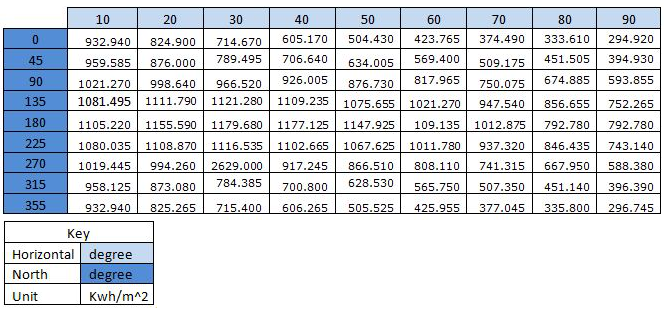
\includegraphics[width=0.9\textwidth]{phase2/group2/figure/table_global_radiation.png}
\caption{LookUp table for the global radiation for Berlin}
\label{fig:rad_table}
\end{figure}